\section{Protolys}

Protolys\footnote{se s. 60 i boken}---från \emph{proto} för proton och forngrekiskans \emph{lúsis} för lossa---innebär att det sker ett utbyte av en eller flera protoner ($\ce{H+}$ joner). Som angivet ovan kommer syror lossa en proton och baser ta emot en.
\begin{exm}
    Låt en syra A som innehåller en väteatom H reagera med vatten. Detta kallas också att den \emph{protolyseras} med vatten:
    \begin{center}
        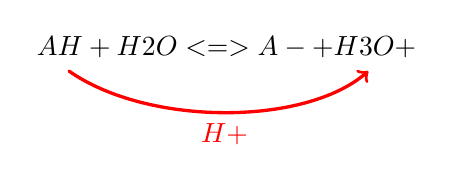
\begin{tikzpicture}
            \node at (0,0) {$\ce{AH + H2O <=> A- + H3O+}$};
            \draw[very thick, color=red, ->, line cap=round] (-2,-0.3) .. controls (-1,-1) and (1,-1) .. node[anchor=north] {$\ce{H+}$} (1.8,-0.3);
        \end{tikzpicture}
    \end{center}
    Något mycket liknande sker när en bas B protolyseras:
    \begin{center}
        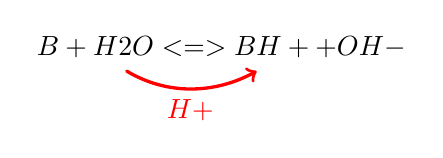
\begin{tikzpicture}
            \node at (0,0) {$\ce{B + H2O <=> BH+ + OH-}$};
            \draw[very thick, color=red, ->, line cap=round] (-1.2,-0.3) .. controls (-0.7,-0.6) and (-0.1,-0.6) .. node[anchor=north] {$\ce{H+}$} (0.45,-0.3);
        \end{tikzpicture}
    \end{center}
\end{exm}

\subsection{Svaga/starka syror och baser}
Man säger att en syra eller en bas kan antingen vara stark eller svag\footnote{se s. 63 samt uppgift 3:29--3.20 i boken}. Detta har faktiskt ingen korrelation med hur mycket den förändrar pH utan det betecknar om reaktionen är fullständig. En syra/bas som protolyseras helt när den placeras i vattelösning kallas stark och alla andra är svaga.

\section{pH och pOH}

Dessa är ett mått på hur syrligt eller basiskt en lösning är. pH är absolut standard med det finns anvädningar för pOH också. Skalan är logaritmisk med bas 10 och går från ca -1 till ca 14. Definitionen för de två storheterna är:
\begin{align*}
    \mathrm{pH} &= -\log_{10}{\ce{[H3O+]}} \\
    \mathrm{pOH} &= -\log_{10}{\ce{[OH^-]}}
\end{align*}
Ju större pH är desto mer basiskt och ju mindre den är desto mer syrligt. En neutral lösning har pH 7, då är $\ce{[H3O+] = [OH^-]}$. För att beräkna den ena från den andra vet vi även detta samband:
\[
    \mathrm{pH + pOH} = 14
\]

\section{Syra- och baskonstanten}
Mycket likt jämviktskonstanten $K$ finns den en så kallad \emph{syrakonstant} $K_a$ och en \emph{baskonstant} $K_b$. Dessa beskriver hur fullständig en syra/bas protolyseras. Dessa värde existerar även för amfolyter---ämnen som är både syra och bas---och bestämmer då om de hellre reagerar som syra eller bas. Dessa värde är som $K$ för för protolysen men man bortser från [$\ce{H2O}$] alltså ser det ut såhär:
\begin{align*}
    K &= \frac{\mathrm{[Bas]} \cdot [\ce{H3O+}]}{\cancel{\ce{[H2O]}} \cdot \mathrm{[Syra]}} \\
    K_a &= \frac{\mathrm{[Bas]} \cdot [\ce{H3O+}]}{\mathrm{[Syra]}} 
\end{align*}
för en syra och följande för en bas:\begin{align*}
    K &= \frac{\mathrm{[Syra]} \cdot [\ce{OH^-}]}{\cancel{\ce{[H2O]}} \cdot \mathrm{[Bas]}} \\
    K_b&= \frac{\mathrm{[Syra]} \cdot [\ce{OH^-}]}{\mathrm{[Bas]}} 
\end{align*}

\subsection{Räkna med syra- och baskonstanten}
Man räknar på dessa konstanter ungefär som man räknar med $K$ (se \vref{sec:räknak}). Skillnaden är att du kommer veta $K_a \text{ eller } K_b$ i förväg från en tabell. Du kan sedan utnyttja detta för att ställa upp jämvikten med tidigare angivna tabeller för att sedan beräkna $\ce{[H3O+] \text{ eller } [OH^-]}$ i en lösning som i sin tur kan leda till pH. Detta är viktigt för att det fungerar även för svaga syror och baser

\subsection{Joner som syra eller bas}
Ibland kan vissa joner från olika salter agera som syror eller baser. Man kan bestämma detta genom att dela upp saltet i dess beståndsdelar. Efter denna uppdelning kan man kolla upp $K_a$ och $K_b$ för dessa joner och avgöra om de reagerar som syra/bas och vilket av dem isåfall. Därefter är logiken för pH exakt samma som för ''vanliga'' syror.

\section{Titrering}
\begin{wrapfigure}{l}{2cm}
    \vspace{-0.8cm}
    % \centering
    \tcbox{\begin{tikzpicture}[scale=0.6, every path/.style={rounded corners=0.5pt}]
        \coordinate (origin) at (0,0);
        \def\byrettwidth{0.2}
        \def\wateroffset{1}
        \coordinate (waterline) at (0,-\wateroffset);
        \def\byrettlength{2.85}
        \coordinate (bottom) at (0,-\byrettlength);
        \def\tiptopwidth{0.08}
        \def\tipbottomwidth{0.03}
        \def\tiplength{0.3}
        \coordinate (tip) at ($(bottom)+(0,-\tiplength)$);

        % wave
        \draw[thick, domain=-\byrettwidth:\byrettwidth, color=cyan!80!blue] plot [samples=50, sharp corners] (\x, {0.015*sin((40*\x) r)-\wateroffset});
        % water fill
        \fill[color=cyan!80!blue, fill opacity=0.4] plot [samples=50, sharp corners, domain=-\byrettwidth:\byrettwidth] (\x, {0.015*sin((40*\x) r)-\wateroffset}) [rounded corners=0.5pt] -- ($(bottom)+(\byrettwidth,0)$) -- ($(bottom)+(\tiptopwidth,0)$) -- ($(tip)+(\tipbottomwidth,0)$) -- ($(tip)+(-\tipbottomwidth,0)$) -- ($(bottom)+(-\tiptopwidth,0)$) -- ($(bottom)+(-\byrettwidth,0)$) [sharp corners] -- cycle;
        % shape
        \draw[thick] ($(origin)+(-\byrettwidth,0)$) -- ($(origin)+(\byrettwidth,0)$) -- ($(bottom)+(\byrettwidth,0)$) -- ($(bottom)+(\tiptopwidth,0)$) -- ($(tip)+(\tipbottomwidth,0)$) -- ($(tip)+(-\tipbottomwidth,0)$) -- ($(bottom)+(-\tiptopwidth,0)$) -- ($(bottom)+(-\byrettwidth,0)$) -- cycle;
        % tickmarks
        \def\tickdist{2.95}
        \foreach \x in {0.05,0.3,...,\tickdist}
          \draw[color=red!80!black, thin] ($(-\byrettwidth,-\x)+(0.05,0)$) -- ($(\byrettwidth,-\x)-(0.05,0)$);
        \foreach \y in {0.1,0.35,...,2.7}
        {
            \pgfmathsetmacro\yoffset{\y+0.05}
            \pgfmathsetmacro\yend{\y+0.2}
            \foreach \z in {\y,\yoffset,...,\yend} 
              \draw[color=red!80!black, very thin] ($(-\byrettwidth, -\z)+(0.1,0)$) -- ($(\byrettwidth, -\z)-(0.1,0)$);
        }
        \foreach \t in {0,0.3,...,1}
          \filldraw[thick, color=cyan!80!blue, fill opacity=0.4, rounded corners=0.2pt] ($(tip)+(0,-\t)+(0,-0.05)$) .. controls ($(tip)+(-0.1,-0.2)+(0,-\t)$) and ($(tip)+(0.1,-0.2)+(0,-\t)$) .. cycle;
        
        % beaker
        \def\beakerwidth{0.6}
        \def\beakerdepth{1.5}
        \def\beakery{3.5}
        \def\beakerwater{4.4}
        \filldraw[very thick, color=cyan!80!blue, fill opacity=0.4, domain=-\beakerwidth:\beakerwidth] plot [samples=50, sharp corners] (\x, {0.015*sin((40*\x) r)-\beakerwater+0.1}) [rounded corners=5pt] -- (\beakerwidth,-\beakerwater) -- ($(\beakerwidth,-\beakery)+(0,-\beakerdepth)$) -- ($(-\beakerwidth,-\beakery)+(0,-\beakerdepth)$) -- (-\beakerwidth,-\beakerwater) [sharp corners] -- cycle;
        \draw[very thick, rounded corners=5pt, line cap=round] (-\beakerwidth,-\beakery) -- ($(-\beakerwidth,-\beakery)+(0,-\beakerdepth)$) -- ($(\beakerwidth,-\beakery)+(0,-\beakerdepth)$) -- (\beakerwidth,-\beakery);
    \end{tikzpicture}}
\end{wrapfigure}
Titrering är ett sätt att ta reda på olika egenskaper hos en syra eller en bas. Man kan exempelvis beräkna mängden lösta ämnen i bägaren, pH, $K_a$ eller $K_b$ från en titrering. Processen går ut på att man placerar någonting i en vattenlösning och i denna lösningen droppar man in en annan med en byrett. Det som sitter i bäger kan vara många olika saker. Vi har exemplet från Kemi 1 av ett rakblad som löses i bägare och den titreras med \(\ce{KMnO4}\) för att undersöka hur mycket \emph{titrand} behövdes för att uppnå ekvivalens. Alla titreringar baseras på ekvivalenser. Man vill droppa i titranden till man når en viss ekvivalens. Detta kan vara en fullständig neutralisation, ett slut på vissa reaktanter eller annat liknande. 
\begin{exm}
    \(0.206\, \mathrm{g}\: \text{rakblad löses i } \ce{H2SO4}\). Lösningen späds till 100 ml. 25 ml av lösningen titrerades med \(0.01\, \mathrm{M}\; \ce{KMnO_4}\) (kaliumpermanganat). Det krävdes 18 ml titrand för att nå ekvivalens. Reaktionen ser ut såhär:
    \begin{equation*}
        \ce{5Fe^2+ + KMnO4- + 8H+ -> 4H2O + Mn^2+ + 5Fe^3+}
    \end{equation*}
    \noindent Vi kommer fram till att det behövdes $0.01\, \mathrm{M} \cdot (18 \cdot 10^{-3})\, \mathrm{l} = 1.8 \cdot 10^{-4}\, \mathrm{mol}\: \ce{KMnO4}$ för att reagera med 25 ml av järnlösning. Det finns 5 gånger mer järn än permangant så vi hade därmed $1.8 \cdot 10^{-4} \cdot 5 = 9 \cdot 10^{-4}\, \mathrm{mol} \: \ce{Fe^2+}$ i 25 ml vilket motsvara $9 \cdot 10^{-4} \cdot 4 = 3.6 \cdot 10^{-3} \, \mathrm{mol}$ järn i 100 ml dvs. hela lösninge.
\end{exm}

\subsection{Titrerkurvor}
En titrerkurva är en graf i 2 dimensioner som beskriver hur pH i en vattelösning förändras när en viss volym titrand tillsätts. Den har två viktiga punkter: \emph{halvtitrerpunkten} och \emph{ekvivalenspunkten}. En titrerkurva kan se ut såhär:
\begin{figure*}[h]
    \centering
    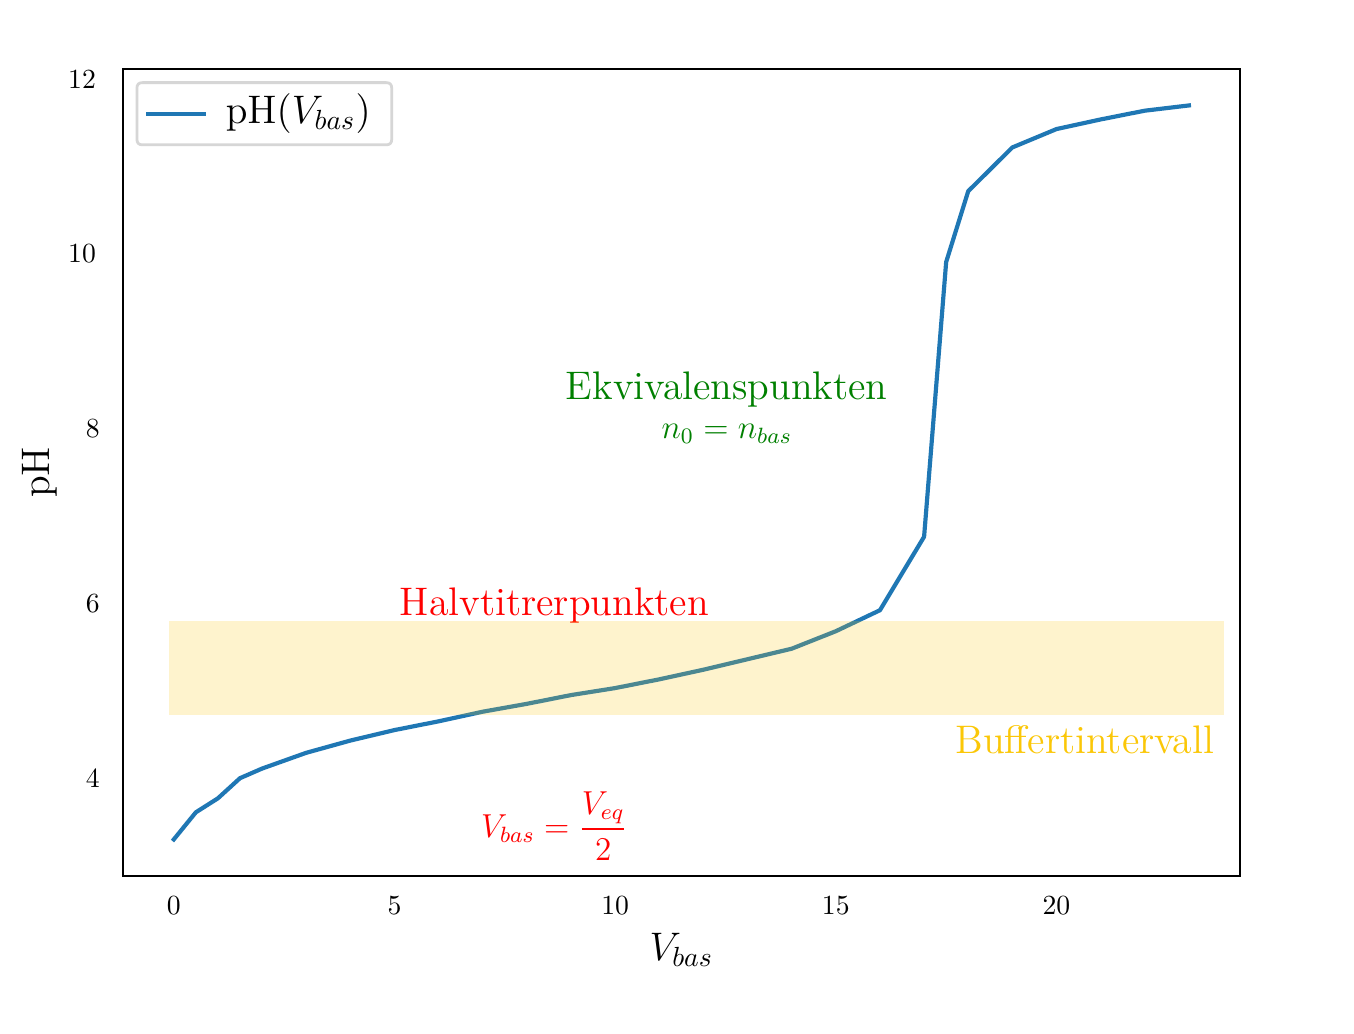
\begin{tikzpicture}[scale=1]
        \hspace{-0.6cm}
        \node at (0,0) [anchor=south west] {\scalebox{1}{%% Creator: Matplotlib, PGF backend
%%
%% To include the figure in your LaTeX document, write
%%   \input{<filename>.pgf}
%%
%% Make sure the required packages are loaded in your preamble
%%   \usepackage{pgf}
%%
%% Also ensure that all the required font packages are loaded; for instance,
%% the lmodern package is sometimes necessary when using math font.
%%   \usepackage{lmodern}
%%
%% Figures using additional raster images can only be included by \input if
%% they are in the same directory as the main LaTeX file. For loading figures
%% from other directories you can use the `import` package
%%   \usepackage{import}
%%
%% and then include the figures with
%%   \import{<path to file>}{<filename>.pgf}
%%
%% Matplotlib used the following preamble
%%   
%%   \usepackage{fontspec}
%%   \setmainfont{DejaVuSerif.ttf}[Path=\detokenize{C:/Users/ziegl/AppData/Roaming/Python/Python310/site-packages/matplotlib/mpl-data/fonts/ttf/}]
%%   \setsansfont{DejaVuSans.ttf}[Path=\detokenize{C:/Users/ziegl/AppData/Roaming/Python/Python310/site-packages/matplotlib/mpl-data/fonts/ttf/}]
%%   \setmonofont{DejaVuSansMono.ttf}[Path=\detokenize{C:/Users/ziegl/AppData/Roaming/Python/Python310/site-packages/matplotlib/mpl-data/fonts/ttf/}]
%%   \makeatletter\@ifpackageloaded{underscore}{}{\usepackage[strings]{underscore}}\makeatother
%%
\begingroup%
\makeatletter%
\begin{pgfpicture}%
\pgfpathrectangle{\pgfpointorigin}{\pgfqpoint{6.400000in}{4.800000in}}%
\pgfusepath{use as bounding box, clip}%
\begin{pgfscope}%
\pgfsetbuttcap%
\pgfsetmiterjoin%
\definecolor{currentfill}{rgb}{1.000000,1.000000,1.000000}%
\pgfsetfillcolor{currentfill}%
\pgfsetlinewidth{0.000000pt}%
\definecolor{currentstroke}{rgb}{1.000000,1.000000,1.000000}%
\pgfsetstrokecolor{currentstroke}%
\pgfsetdash{}{0pt}%
\pgfpathmoveto{\pgfqpoint{0.000000in}{0.000000in}}%
\pgfpathlineto{\pgfqpoint{6.400000in}{0.000000in}}%
\pgfpathlineto{\pgfqpoint{6.400000in}{4.800000in}}%
\pgfpathlineto{\pgfqpoint{0.000000in}{4.800000in}}%
\pgfpathlineto{\pgfqpoint{0.000000in}{0.000000in}}%
\pgfpathclose%
\pgfusepath{fill}%
\end{pgfscope}%
\begin{pgfscope}%
\pgfsetbuttcap%
\pgfsetmiterjoin%
\definecolor{currentfill}{rgb}{1.000000,1.000000,1.000000}%
\pgfsetfillcolor{currentfill}%
\pgfsetlinewidth{0.000000pt}%
\definecolor{currentstroke}{rgb}{0.000000,0.000000,0.000000}%
\pgfsetstrokecolor{currentstroke}%
\pgfsetstrokeopacity{0.000000}%
\pgfsetdash{}{0pt}%
\pgfpathmoveto{\pgfqpoint{0.666911in}{0.603857in}}%
\pgfpathlineto{\pgfqpoint{6.250000in}{0.603857in}}%
\pgfpathlineto{\pgfqpoint{6.250000in}{4.640722in}}%
\pgfpathlineto{\pgfqpoint{0.666911in}{4.640722in}}%
\pgfpathlineto{\pgfqpoint{0.666911in}{0.603857in}}%
\pgfpathclose%
\pgfusepath{fill}%
\end{pgfscope}%
\begin{pgfscope}%
\pgfsetbuttcap%
\pgfsetroundjoin%
\definecolor{currentfill}{rgb}{0.000000,0.000000,0.000000}%
\pgfsetfillcolor{currentfill}%
\pgfsetlinewidth{0.803000pt}%
\definecolor{currentstroke}{rgb}{0.000000,0.000000,0.000000}%
\pgfsetstrokecolor{currentstroke}%
\pgfsetdash{}{0pt}%
\pgfsys@defobject{currentmarker}{\pgfqpoint{0.000000in}{-0.048611in}}{\pgfqpoint{0.000000in}{0.000000in}}{%
\pgfpathmoveto{\pgfqpoint{0.000000in}{0.000000in}}%
\pgfpathlineto{\pgfqpoint{0.000000in}{-0.048611in}}%
\pgfusepath{stroke,fill}%
}%
\begin{pgfscope}%
\pgfsys@transformshift{0.920687in}{0.603857in}%
\pgfsys@useobject{currentmarker}{}%
\end{pgfscope}%
\end{pgfscope}%
\begin{pgfscope}%
\definecolor{textcolor}{rgb}{0.000000,0.000000,0.000000}%
\pgfsetstrokecolor{textcolor}%
\pgfsetfillcolor{textcolor}%
\pgftext[x=0.920687in,y=0.506635in,,top]{\color{textcolor}\rmfamily\fontsize{10.000000}{12.000000}\selectfont 0}%
\end{pgfscope}%
\begin{pgfscope}%
\pgfsetbuttcap%
\pgfsetroundjoin%
\definecolor{currentfill}{rgb}{0.000000,0.000000,0.000000}%
\pgfsetfillcolor{currentfill}%
\pgfsetlinewidth{0.803000pt}%
\definecolor{currentstroke}{rgb}{0.000000,0.000000,0.000000}%
\pgfsetstrokecolor{currentstroke}%
\pgfsetdash{}{0pt}%
\pgfsys@defobject{currentmarker}{\pgfqpoint{0.000000in}{-0.048611in}}{\pgfqpoint{0.000000in}{0.000000in}}{%
\pgfpathmoveto{\pgfqpoint{0.000000in}{0.000000in}}%
\pgfpathlineto{\pgfqpoint{0.000000in}{-0.048611in}}%
\pgfusepath{stroke,fill}%
}%
\begin{pgfscope}%
\pgfsys@transformshift{2.024065in}{0.603857in}%
\pgfsys@useobject{currentmarker}{}%
\end{pgfscope}%
\end{pgfscope}%
\begin{pgfscope}%
\definecolor{textcolor}{rgb}{0.000000,0.000000,0.000000}%
\pgfsetstrokecolor{textcolor}%
\pgfsetfillcolor{textcolor}%
\pgftext[x=2.024065in,y=0.506635in,,top]{\color{textcolor}\rmfamily\fontsize{10.000000}{12.000000}\selectfont 5}%
\end{pgfscope}%
\begin{pgfscope}%
\pgfsetbuttcap%
\pgfsetroundjoin%
\definecolor{currentfill}{rgb}{0.000000,0.000000,0.000000}%
\pgfsetfillcolor{currentfill}%
\pgfsetlinewidth{0.803000pt}%
\definecolor{currentstroke}{rgb}{0.000000,0.000000,0.000000}%
\pgfsetstrokecolor{currentstroke}%
\pgfsetdash{}{0pt}%
\pgfsys@defobject{currentmarker}{\pgfqpoint{0.000000in}{-0.048611in}}{\pgfqpoint{0.000000in}{0.000000in}}{%
\pgfpathmoveto{\pgfqpoint{0.000000in}{0.000000in}}%
\pgfpathlineto{\pgfqpoint{0.000000in}{-0.048611in}}%
\pgfusepath{stroke,fill}%
}%
\begin{pgfscope}%
\pgfsys@transformshift{3.127442in}{0.603857in}%
\pgfsys@useobject{currentmarker}{}%
\end{pgfscope}%
\end{pgfscope}%
\begin{pgfscope}%
\definecolor{textcolor}{rgb}{0.000000,0.000000,0.000000}%
\pgfsetstrokecolor{textcolor}%
\pgfsetfillcolor{textcolor}%
\pgftext[x=3.127442in,y=0.506635in,,top]{\color{textcolor}\rmfamily\fontsize{10.000000}{12.000000}\selectfont 10}%
\end{pgfscope}%
\begin{pgfscope}%
\pgfsetbuttcap%
\pgfsetroundjoin%
\definecolor{currentfill}{rgb}{0.000000,0.000000,0.000000}%
\pgfsetfillcolor{currentfill}%
\pgfsetlinewidth{0.803000pt}%
\definecolor{currentstroke}{rgb}{0.000000,0.000000,0.000000}%
\pgfsetstrokecolor{currentstroke}%
\pgfsetdash{}{0pt}%
\pgfsys@defobject{currentmarker}{\pgfqpoint{0.000000in}{-0.048611in}}{\pgfqpoint{0.000000in}{0.000000in}}{%
\pgfpathmoveto{\pgfqpoint{0.000000in}{0.000000in}}%
\pgfpathlineto{\pgfqpoint{0.000000in}{-0.048611in}}%
\pgfusepath{stroke,fill}%
}%
\begin{pgfscope}%
\pgfsys@transformshift{4.230819in}{0.603857in}%
\pgfsys@useobject{currentmarker}{}%
\end{pgfscope}%
\end{pgfscope}%
\begin{pgfscope}%
\definecolor{textcolor}{rgb}{0.000000,0.000000,0.000000}%
\pgfsetstrokecolor{textcolor}%
\pgfsetfillcolor{textcolor}%
\pgftext[x=4.230819in,y=0.506635in,,top]{\color{textcolor}\rmfamily\fontsize{10.000000}{12.000000}\selectfont 15}%
\end{pgfscope}%
\begin{pgfscope}%
\pgfsetbuttcap%
\pgfsetroundjoin%
\definecolor{currentfill}{rgb}{0.000000,0.000000,0.000000}%
\pgfsetfillcolor{currentfill}%
\pgfsetlinewidth{0.803000pt}%
\definecolor{currentstroke}{rgb}{0.000000,0.000000,0.000000}%
\pgfsetstrokecolor{currentstroke}%
\pgfsetdash{}{0pt}%
\pgfsys@defobject{currentmarker}{\pgfqpoint{0.000000in}{-0.048611in}}{\pgfqpoint{0.000000in}{0.000000in}}{%
\pgfpathmoveto{\pgfqpoint{0.000000in}{0.000000in}}%
\pgfpathlineto{\pgfqpoint{0.000000in}{-0.048611in}}%
\pgfusepath{stroke,fill}%
}%
\begin{pgfscope}%
\pgfsys@transformshift{5.334197in}{0.603857in}%
\pgfsys@useobject{currentmarker}{}%
\end{pgfscope}%
\end{pgfscope}%
\begin{pgfscope}%
\definecolor{textcolor}{rgb}{0.000000,0.000000,0.000000}%
\pgfsetstrokecolor{textcolor}%
\pgfsetfillcolor{textcolor}%
\pgftext[x=5.334197in,y=0.506635in,,top]{\color{textcolor}\rmfamily\fontsize{10.000000}{12.000000}\selectfont 20}%
\end{pgfscope}%
\begin{pgfscope}%
\definecolor{textcolor}{rgb}{0.000000,0.000000,0.000000}%
\pgfsetstrokecolor{textcolor}%
\pgfsetfillcolor{textcolor}%
\pgftext[x=3.458455in,y=0.316667in,,top]{\color{textcolor}\rmfamily\fontsize{10.000000}{12.000000}\selectfont \Large{\(\displaystyle V_{bas}\)}}%
\end{pgfscope}%
\begin{pgfscope}%
\pgfsetbuttcap%
\pgfsetroundjoin%
\definecolor{currentfill}{rgb}{0.000000,0.000000,0.000000}%
\pgfsetfillcolor{currentfill}%
\pgfsetlinewidth{0.803000pt}%
\definecolor{currentstroke}{rgb}{0.000000,0.000000,0.000000}%
\pgfsetstrokecolor{currentstroke}%
\pgfsetdash{}{0pt}%
\pgfsys@defobject{currentmarker}{\pgfqpoint{-0.048611in}{0.000000in}}{\pgfqpoint{-0.000000in}{0.000000in}}{%
\pgfpathmoveto{\pgfqpoint{-0.000000in}{0.000000in}}%
\pgfpathlineto{\pgfqpoint{-0.048611in}{0.000000in}}%
\pgfusepath{stroke,fill}%
}%
\begin{pgfscope}%
\pgfsys@transformshift{0.666911in}{1.097913in}%
\pgfsys@useobject{currentmarker}{}%
\end{pgfscope}%
\end{pgfscope}%
\begin{pgfscope}%
\definecolor{textcolor}{rgb}{0.000000,0.000000,0.000000}%
\pgfsetstrokecolor{textcolor}%
\pgfsetfillcolor{textcolor}%
\pgftext[x=0.481323in, y=1.045151in, left, base]{\color{textcolor}\rmfamily\fontsize{10.000000}{12.000000}\selectfont 4}%
\end{pgfscope}%
\begin{pgfscope}%
\pgfsetbuttcap%
\pgfsetroundjoin%
\definecolor{currentfill}{rgb}{0.000000,0.000000,0.000000}%
\pgfsetfillcolor{currentfill}%
\pgfsetlinewidth{0.803000pt}%
\definecolor{currentstroke}{rgb}{0.000000,0.000000,0.000000}%
\pgfsetstrokecolor{currentstroke}%
\pgfsetdash{}{0pt}%
\pgfsys@defobject{currentmarker}{\pgfqpoint{-0.048611in}{0.000000in}}{\pgfqpoint{-0.000000in}{0.000000in}}{%
\pgfpathmoveto{\pgfqpoint{-0.000000in}{0.000000in}}%
\pgfpathlineto{\pgfqpoint{-0.048611in}{0.000000in}}%
\pgfusepath{stroke,fill}%
}%
\begin{pgfscope}%
\pgfsys@transformshift{0.666911in}{1.972734in}%
\pgfsys@useobject{currentmarker}{}%
\end{pgfscope}%
\end{pgfscope}%
\begin{pgfscope}%
\definecolor{textcolor}{rgb}{0.000000,0.000000,0.000000}%
\pgfsetstrokecolor{textcolor}%
\pgfsetfillcolor{textcolor}%
\pgftext[x=0.481323in, y=1.919973in, left, base]{\color{textcolor}\rmfamily\fontsize{10.000000}{12.000000}\selectfont 6}%
\end{pgfscope}%
\begin{pgfscope}%
\pgfsetbuttcap%
\pgfsetroundjoin%
\definecolor{currentfill}{rgb}{0.000000,0.000000,0.000000}%
\pgfsetfillcolor{currentfill}%
\pgfsetlinewidth{0.803000pt}%
\definecolor{currentstroke}{rgb}{0.000000,0.000000,0.000000}%
\pgfsetstrokecolor{currentstroke}%
\pgfsetdash{}{0pt}%
\pgfsys@defobject{currentmarker}{\pgfqpoint{-0.048611in}{0.000000in}}{\pgfqpoint{-0.000000in}{0.000000in}}{%
\pgfpathmoveto{\pgfqpoint{-0.000000in}{0.000000in}}%
\pgfpathlineto{\pgfqpoint{-0.048611in}{0.000000in}}%
\pgfusepath{stroke,fill}%
}%
\begin{pgfscope}%
\pgfsys@transformshift{0.666911in}{2.847556in}%
\pgfsys@useobject{currentmarker}{}%
\end{pgfscope}%
\end{pgfscope}%
\begin{pgfscope}%
\definecolor{textcolor}{rgb}{0.000000,0.000000,0.000000}%
\pgfsetstrokecolor{textcolor}%
\pgfsetfillcolor{textcolor}%
\pgftext[x=0.481323in, y=2.794794in, left, base]{\color{textcolor}\rmfamily\fontsize{10.000000}{12.000000}\selectfont 8}%
\end{pgfscope}%
\begin{pgfscope}%
\pgfsetbuttcap%
\pgfsetroundjoin%
\definecolor{currentfill}{rgb}{0.000000,0.000000,0.000000}%
\pgfsetfillcolor{currentfill}%
\pgfsetlinewidth{0.803000pt}%
\definecolor{currentstroke}{rgb}{0.000000,0.000000,0.000000}%
\pgfsetstrokecolor{currentstroke}%
\pgfsetdash{}{0pt}%
\pgfsys@defobject{currentmarker}{\pgfqpoint{-0.048611in}{0.000000in}}{\pgfqpoint{-0.000000in}{0.000000in}}{%
\pgfpathmoveto{\pgfqpoint{-0.000000in}{0.000000in}}%
\pgfpathlineto{\pgfqpoint{-0.048611in}{0.000000in}}%
\pgfusepath{stroke,fill}%
}%
\begin{pgfscope}%
\pgfsys@transformshift{0.666911in}{3.722378in}%
\pgfsys@useobject{currentmarker}{}%
\end{pgfscope}%
\end{pgfscope}%
\begin{pgfscope}%
\definecolor{textcolor}{rgb}{0.000000,0.000000,0.000000}%
\pgfsetstrokecolor{textcolor}%
\pgfsetfillcolor{textcolor}%
\pgftext[x=0.392958in, y=3.669616in, left, base]{\color{textcolor}\rmfamily\fontsize{10.000000}{12.000000}\selectfont 10}%
\end{pgfscope}%
\begin{pgfscope}%
\pgfsetbuttcap%
\pgfsetroundjoin%
\definecolor{currentfill}{rgb}{0.000000,0.000000,0.000000}%
\pgfsetfillcolor{currentfill}%
\pgfsetlinewidth{0.803000pt}%
\definecolor{currentstroke}{rgb}{0.000000,0.000000,0.000000}%
\pgfsetstrokecolor{currentstroke}%
\pgfsetdash{}{0pt}%
\pgfsys@defobject{currentmarker}{\pgfqpoint{-0.048611in}{0.000000in}}{\pgfqpoint{-0.000000in}{0.000000in}}{%
\pgfpathmoveto{\pgfqpoint{-0.000000in}{0.000000in}}%
\pgfpathlineto{\pgfqpoint{-0.048611in}{0.000000in}}%
\pgfusepath{stroke,fill}%
}%
\begin{pgfscope}%
\pgfsys@transformshift{0.666911in}{4.597199in}%
\pgfsys@useobject{currentmarker}{}%
\end{pgfscope}%
\end{pgfscope}%
\begin{pgfscope}%
\definecolor{textcolor}{rgb}{0.000000,0.000000,0.000000}%
\pgfsetstrokecolor{textcolor}%
\pgfsetfillcolor{textcolor}%
\pgftext[x=0.392958in, y=4.544438in, left, base]{\color{textcolor}\rmfamily\fontsize{10.000000}{12.000000}\selectfont 12}%
\end{pgfscope}%
\begin{pgfscope}%
\definecolor{textcolor}{rgb}{0.000000,0.000000,0.000000}%
\pgfsetstrokecolor{textcolor}%
\pgfsetfillcolor{textcolor}%
\pgftext[x=0.337402in,y=2.622289in,,bottom,rotate=90.000000]{\color{textcolor}\rmfamily\fontsize{10.000000}{12.000000}\selectfont \Large{pH}}%
\end{pgfscope}%
\begin{pgfscope}%
\pgfpathrectangle{\pgfqpoint{0.666911in}{0.603857in}}{\pgfqpoint{5.583089in}{4.036865in}}%
\pgfusepath{clip}%
\pgfsetrectcap%
\pgfsetroundjoin%
\pgfsetlinewidth{1.505625pt}%
\definecolor{currentstroke}{rgb}{0.121569,0.466667,0.705882}%
\pgfsetstrokecolor{currentstroke}%
\pgfsetdash{}{0pt}%
\pgfpathmoveto{\pgfqpoint{0.920687in}{0.787351in}}%
\pgfpathlineto{\pgfqpoint{1.031025in}{0.922948in}}%
\pgfpathlineto{\pgfqpoint{1.141363in}{0.992934in}}%
\pgfpathlineto{\pgfqpoint{1.251701in}{1.093539in}}%
\pgfpathlineto{\pgfqpoint{1.362038in}{1.141654in}}%
\pgfpathlineto{\pgfqpoint{1.582714in}{1.220388in}}%
\pgfpathlineto{\pgfqpoint{1.803389in}{1.281625in}}%
\pgfpathlineto{\pgfqpoint{2.024065in}{1.334114in}}%
\pgfpathlineto{\pgfqpoint{2.244740in}{1.377856in}}%
\pgfpathlineto{\pgfqpoint{2.465416in}{1.425971in}}%
\pgfpathlineto{\pgfqpoint{2.686091in}{1.465338in}}%
\pgfpathlineto{\pgfqpoint{2.906767in}{1.509079in}}%
\pgfpathlineto{\pgfqpoint{3.127442in}{1.544072in}}%
\pgfpathlineto{\pgfqpoint{3.348118in}{1.587813in}}%
\pgfpathlineto{\pgfqpoint{3.568793in}{1.635928in}}%
\pgfpathlineto{\pgfqpoint{3.789468in}{1.688417in}}%
\pgfpathlineto{\pgfqpoint{4.010144in}{1.740907in}}%
\pgfpathlineto{\pgfqpoint{4.230819in}{1.828389in}}%
\pgfpathlineto{\pgfqpoint{4.451495in}{1.933367in}}%
\pgfpathlineto{\pgfqpoint{4.672170in}{2.300792in}}%
\pgfpathlineto{\pgfqpoint{4.782508in}{3.674262in}}%
\pgfpathlineto{\pgfqpoint{4.892846in}{4.028565in}}%
\pgfpathlineto{\pgfqpoint{5.113521in}{4.247271in}}%
\pgfpathlineto{\pgfqpoint{5.334197in}{4.339127in}}%
\pgfpathlineto{\pgfqpoint{5.554872in}{4.387242in}}%
\pgfpathlineto{\pgfqpoint{5.775548in}{4.430983in}}%
\pgfpathlineto{\pgfqpoint{5.996223in}{4.457228in}}%
\pgfusepath{stroke}%
\end{pgfscope}%
\begin{pgfscope}%
\pgfpathrectangle{\pgfqpoint{0.666911in}{0.603857in}}{\pgfqpoint{5.583089in}{4.036865in}}%
\pgfusepath{clip}%
\pgfsetbuttcap%
\pgfsetroundjoin%
\definecolor{currentfill}{rgb}{0.000000,0.500000,0.000000}%
\pgfsetfillcolor{currentfill}%
\pgfsetlinewidth{1.003750pt}%
\definecolor{currentstroke}{rgb}{0.000000,0.500000,0.000000}%
\pgfsetstrokecolor{currentstroke}%
\pgfsetdash{}{0pt}%
\pgfsys@defobject{currentmarker}{\pgfqpoint{-0.041667in}{-0.041667in}}{\pgfqpoint{0.041667in}{0.041667in}}{%
\pgfpathmoveto{\pgfqpoint{0.000000in}{-0.041667in}}%
\pgfpathcurveto{\pgfqpoint{0.011050in}{-0.041667in}}{\pgfqpoint{0.021649in}{-0.037276in}}{\pgfqpoint{0.029463in}{-0.029463in}}%
\pgfpathcurveto{\pgfqpoint{0.037276in}{-0.021649in}}{\pgfqpoint{0.041667in}{-0.011050in}}{\pgfqpoint{0.041667in}{0.000000in}}%
\pgfpathcurveto{\pgfqpoint{0.041667in}{0.011050in}}{\pgfqpoint{0.037276in}{0.021649in}}{\pgfqpoint{0.029463in}{0.029463in}}%
\pgfpathcurveto{\pgfqpoint{0.021649in}{0.037276in}}{\pgfqpoint{0.011050in}{0.041667in}}{\pgfqpoint{0.000000in}{0.041667in}}%
\pgfpathcurveto{\pgfqpoint{-0.011050in}{0.041667in}}{\pgfqpoint{-0.021649in}{0.037276in}}{\pgfqpoint{-0.029463in}{0.029463in}}%
\pgfpathcurveto{\pgfqpoint{-0.037276in}{0.021649in}}{\pgfqpoint{-0.041667in}{0.011050in}}{\pgfqpoint{-0.041667in}{0.000000in}}%
\pgfpathcurveto{\pgfqpoint{-0.041667in}{-0.011050in}}{\pgfqpoint{-0.037276in}{-0.021649in}}{\pgfqpoint{-0.029463in}{-0.029463in}}%
\pgfpathcurveto{\pgfqpoint{-0.021649in}{-0.037276in}}{\pgfqpoint{-0.011050in}{-0.041667in}}{\pgfqpoint{0.000000in}{-0.041667in}}%
\pgfpathlineto{\pgfqpoint{0.000000in}{-0.041667in}}%
\pgfpathclose%
\pgfusepath{stroke,fill}%
}%
\begin{pgfscope}%
\pgfsys@transformshift{4.727339in}{2.987527in}%
\pgfsys@useobject{currentmarker}{}%
\end{pgfscope}%
\end{pgfscope}%
\begin{pgfscope}%
\pgfpathrectangle{\pgfqpoint{0.666911in}{0.603857in}}{\pgfqpoint{5.583089in}{4.036865in}}%
\pgfusepath{clip}%
\pgfsetrectcap%
\pgfsetroundjoin%
\pgfsetlinewidth{1.505625pt}%
\definecolor{currentstroke}{rgb}{1.000000,0.000000,0.000000}%
\pgfsetstrokecolor{currentstroke}%
\pgfsetdash{}{0pt}%
\pgfpathmoveto{\pgfqpoint{2.824013in}{1.492676in}}%
\pgfusepath{stroke}%
\end{pgfscope}%
\begin{pgfscope}%
\pgfpathrectangle{\pgfqpoint{0.666911in}{0.603857in}}{\pgfqpoint{5.583089in}{4.036865in}}%
\pgfusepath{clip}%
\pgfsetbuttcap%
\pgfsetroundjoin%
\definecolor{currentfill}{rgb}{1.000000,0.000000,0.000000}%
\pgfsetfillcolor{currentfill}%
\pgfsetlinewidth{1.003750pt}%
\definecolor{currentstroke}{rgb}{1.000000,0.000000,0.000000}%
\pgfsetstrokecolor{currentstroke}%
\pgfsetdash{}{0pt}%
\pgfsys@defobject{currentmarker}{\pgfqpoint{-0.041667in}{-0.041667in}}{\pgfqpoint{0.041667in}{0.041667in}}{%
\pgfpathmoveto{\pgfqpoint{0.000000in}{-0.041667in}}%
\pgfpathcurveto{\pgfqpoint{0.011050in}{-0.041667in}}{\pgfqpoint{0.021649in}{-0.037276in}}{\pgfqpoint{0.029463in}{-0.029463in}}%
\pgfpathcurveto{\pgfqpoint{0.037276in}{-0.021649in}}{\pgfqpoint{0.041667in}{-0.011050in}}{\pgfqpoint{0.041667in}{0.000000in}}%
\pgfpathcurveto{\pgfqpoint{0.041667in}{0.011050in}}{\pgfqpoint{0.037276in}{0.021649in}}{\pgfqpoint{0.029463in}{0.029463in}}%
\pgfpathcurveto{\pgfqpoint{0.021649in}{0.037276in}}{\pgfqpoint{0.011050in}{0.041667in}}{\pgfqpoint{0.000000in}{0.041667in}}%
\pgfpathcurveto{\pgfqpoint{-0.011050in}{0.041667in}}{\pgfqpoint{-0.021649in}{0.037276in}}{\pgfqpoint{-0.029463in}{0.029463in}}%
\pgfpathcurveto{\pgfqpoint{-0.037276in}{0.021649in}}{\pgfqpoint{-0.041667in}{0.011050in}}{\pgfqpoint{-0.041667in}{0.000000in}}%
\pgfpathcurveto{\pgfqpoint{-0.041667in}{-0.011050in}}{\pgfqpoint{-0.037276in}{-0.021649in}}{\pgfqpoint{-0.029463in}{-0.029463in}}%
\pgfpathcurveto{\pgfqpoint{-0.021649in}{-0.037276in}}{\pgfqpoint{-0.011050in}{-0.041667in}}{\pgfqpoint{0.000000in}{-0.041667in}}%
\pgfpathlineto{\pgfqpoint{0.000000in}{-0.041667in}}%
\pgfpathclose%
\pgfusepath{stroke,fill}%
}%
\begin{pgfscope}%
\pgfsys@transformshift{2.824013in}{1.492676in}%
\pgfsys@useobject{currentmarker}{}%
\end{pgfscope}%
\end{pgfscope}%
\begin{pgfscope}%
\pgfsetrectcap%
\pgfsetmiterjoin%
\pgfsetlinewidth{0.803000pt}%
\definecolor{currentstroke}{rgb}{0.000000,0.000000,0.000000}%
\pgfsetstrokecolor{currentstroke}%
\pgfsetdash{}{0pt}%
\pgfpathmoveto{\pgfqpoint{0.666911in}{0.603857in}}%
\pgfpathlineto{\pgfqpoint{0.666911in}{4.640722in}}%
\pgfusepath{stroke}%
\end{pgfscope}%
\begin{pgfscope}%
\pgfsetrectcap%
\pgfsetmiterjoin%
\pgfsetlinewidth{0.803000pt}%
\definecolor{currentstroke}{rgb}{0.000000,0.000000,0.000000}%
\pgfsetstrokecolor{currentstroke}%
\pgfsetdash{}{0pt}%
\pgfpathmoveto{\pgfqpoint{6.250000in}{0.603857in}}%
\pgfpathlineto{\pgfqpoint{6.250000in}{4.640722in}}%
\pgfusepath{stroke}%
\end{pgfscope}%
\begin{pgfscope}%
\pgfsetrectcap%
\pgfsetmiterjoin%
\pgfsetlinewidth{0.803000pt}%
\definecolor{currentstroke}{rgb}{0.000000,0.000000,0.000000}%
\pgfsetstrokecolor{currentstroke}%
\pgfsetdash{}{0pt}%
\pgfpathmoveto{\pgfqpoint{0.666911in}{0.603857in}}%
\pgfpathlineto{\pgfqpoint{6.250000in}{0.603857in}}%
\pgfusepath{stroke}%
\end{pgfscope}%
\begin{pgfscope}%
\pgfsetrectcap%
\pgfsetmiterjoin%
\pgfsetlinewidth{0.803000pt}%
\definecolor{currentstroke}{rgb}{0.000000,0.000000,0.000000}%
\pgfsetstrokecolor{currentstroke}%
\pgfsetdash{}{0pt}%
\pgfpathmoveto{\pgfqpoint{0.666911in}{4.640722in}}%
\pgfpathlineto{\pgfqpoint{6.250000in}{4.640722in}}%
\pgfusepath{stroke}%
\end{pgfscope}%
\begin{pgfscope}%
\definecolor{textcolor}{rgb}{0.000000,0.501961,0.000000}%
\pgfsetstrokecolor{textcolor}%
\pgfsetfillcolor{textcolor}%
\pgftext[x=3.685673in,y=2.987527in,,base]{\color{textcolor}\rmfamily\fontsize{10.000000}{12.000000}\selectfont \Large{Ekvivalenspunkten}}%
\end{pgfscope}%
\begin{pgfscope}%
\definecolor{textcolor}{rgb}{0.000000,0.501961,0.000000}%
\pgfsetstrokecolor{textcolor}%
\pgfsetfillcolor{textcolor}%
\pgftext[x=3.685673in,y=2.793083in,,base]{\color{textcolor}\rmfamily\fontsize{10.000000}{12.000000}\selectfont \large{\(\displaystyle n_{0} = n_{bas}\)}}%
\end{pgfscope}%
\begin{pgfscope}%
\definecolor{textcolor}{rgb}{1.000000,0.000000,0.000000}%
\pgfsetstrokecolor{textcolor}%
\pgfsetfillcolor{textcolor}%
\pgftext[x=2.824013in,y=1.909343in,,base]{\color{textcolor}\rmfamily\fontsize{10.000000}{12.000000}\selectfont \Large{Halvtitrerpunkten}}%
\end{pgfscope}%
\begin{pgfscope}%
\definecolor{textcolor}{rgb}{1.000000,0.000000,0.000000}%
\pgfsetstrokecolor{textcolor}%
\pgfsetfillcolor{textcolor}%
\pgftext[x=2.824013in,y=0.798231in,,base]{\color{textcolor}\rmfamily\fontsize{10.000000}{12.000000}\selectfont \large{\(\displaystyle V_{bas} = \frac{V_{eq}}{2}\)}}%
\end{pgfscope}%
\begin{pgfscope}%
\pgfsetbuttcap%
\pgfsetmiterjoin%
\definecolor{currentfill}{rgb}{1.000000,1.000000,1.000000}%
\pgfsetfillcolor{currentfill}%
\pgfsetfillopacity{0.800000}%
\pgfsetlinewidth{1.003750pt}%
\definecolor{currentstroke}{rgb}{0.800000,0.800000,0.800000}%
\pgfsetstrokecolor{currentstroke}%
\pgfsetstrokeopacity{0.800000}%
\pgfsetdash{}{0pt}%
\pgfpathmoveto{\pgfqpoint{0.764133in}{4.260166in}}%
\pgfpathlineto{\pgfqpoint{1.982567in}{4.260166in}}%
\pgfpathquadraticcurveto{\pgfqpoint{2.010345in}{4.260166in}}{\pgfqpoint{2.010345in}{4.287944in}}%
\pgfpathlineto{\pgfqpoint{2.010345in}{4.543499in}}%
\pgfpathquadraticcurveto{\pgfqpoint{2.010345in}{4.571277in}}{\pgfqpoint{1.982567in}{4.571277in}}%
\pgfpathlineto{\pgfqpoint{0.764133in}{4.571277in}}%
\pgfpathquadraticcurveto{\pgfqpoint{0.736355in}{4.571277in}}{\pgfqpoint{0.736355in}{4.543499in}}%
\pgfpathlineto{\pgfqpoint{0.736355in}{4.287944in}}%
\pgfpathquadraticcurveto{\pgfqpoint{0.736355in}{4.260166in}}{\pgfqpoint{0.764133in}{4.260166in}}%
\pgfpathlineto{\pgfqpoint{0.764133in}{4.260166in}}%
\pgfpathclose%
\pgfusepath{stroke,fill}%
\end{pgfscope}%
\begin{pgfscope}%
\pgfsetrectcap%
\pgfsetroundjoin%
\pgfsetlinewidth{1.505625pt}%
\definecolor{currentstroke}{rgb}{0.121569,0.466667,0.705882}%
\pgfsetstrokecolor{currentstroke}%
\pgfsetdash{}{0pt}%
\pgfpathmoveto{\pgfqpoint{0.791911in}{4.414333in}}%
\pgfpathlineto{\pgfqpoint{0.930799in}{4.414333in}}%
\pgfpathlineto{\pgfqpoint{1.069688in}{4.414333in}}%
\pgfusepath{stroke}%
\end{pgfscope}%
\begin{pgfscope}%
\definecolor{textcolor}{rgb}{0.000000,0.000000,0.000000}%
\pgfsetstrokecolor{textcolor}%
\pgfsetfillcolor{textcolor}%
\pgftext[x=1.180799in,y=4.365722in,left,base]{\color{textcolor}\rmfamily\fontsize{10.000000}{12.000000}\selectfont \Large{\(\displaystyle \mathrm{pH}(V_{bas})\)}}%
\end{pgfscope}%
\end{pgfpicture}%
\makeatother%
\endgroup%
}};
        \fill[color=yellow!80!red, fill opacity=0.2] (2.4,4.9) rectangle (15.8,3.7) node[anchor=north east, fill opacity=1] {\Large{Buffertintervall}};
    \end{tikzpicture}
    \caption{Titrerkurva}
    \label{fig:titrerkurva}
\end{figure*}